\subsubsection{Случай Лагранжа}

\begin{wrapfigure}{l}{0.5\textwidth}
  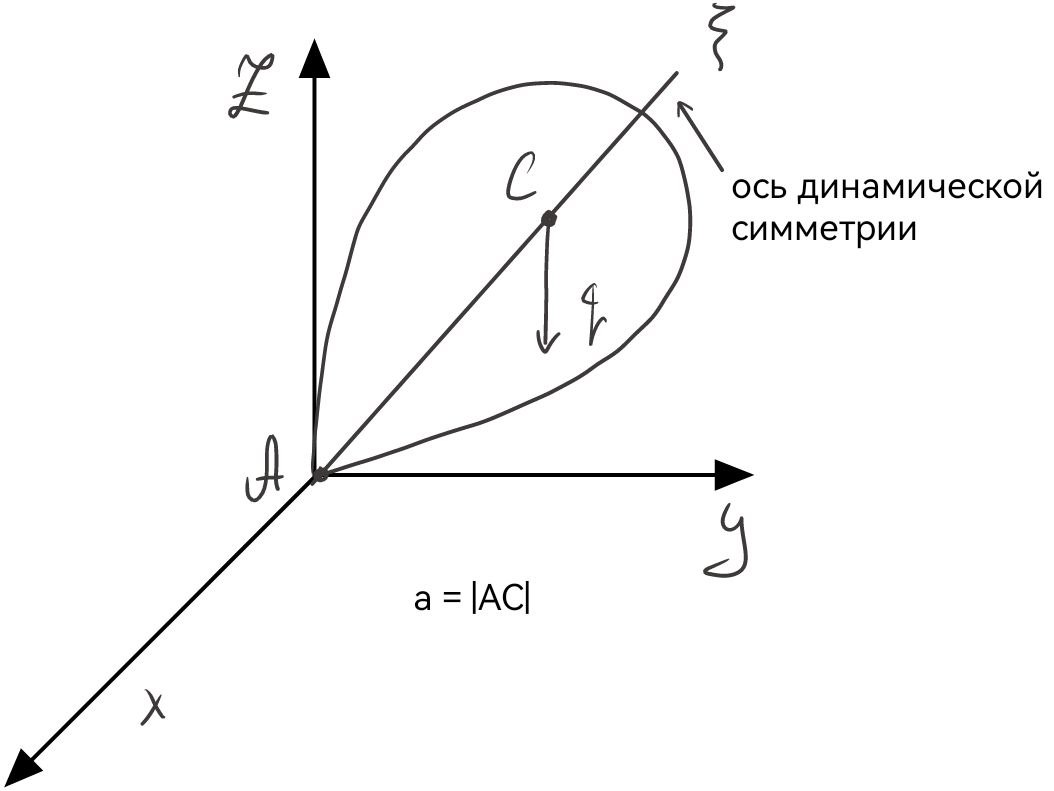
\includegraphics[width=0.8\linewidth]{images/лекция_10_1.jpeg}
\end{wrapfigure}

\underline{Требования}:\\
\begin{enumerate}
  \item Динамическая симметрия: A = B $\neq$ C
  \item Движение в однородном поле (например, однородное поле тяжести $\Longrightarrow$ в каком-то направлении нет момента сил $\Longrightarrow$ первый интеграл)
  \item $M_A$ не дает проекции на ось динамической симметрии (центр масс лежит на оси динамической симметрии)
\end{enumerate}              


\underline{Интеграл энергии}\\
Пусть P --- потенциальная энергия, p и q --- проекции угловой скорости волчка на плоскость динамической симметрии, тогда закон сохранения энергии можно записать в виде
\[
\dfrac{1}{2}(A(p^2 + q^2) + Cr^2 + P a \cos{\Theta} = E
\]
Т.к. $Cr^2 = const$
\[
A(p^2 + q^2) + 2P a \cos{\Theta} = 2E - Cr^2 = 2E'
\]

\underline{Сохранение проекции момента импульса в случае Лагранжа}\\
Пусть $K^z$ --- проекция момента импульса на ось z.\\

Тогда
\[
\left(u_1(\Theta) \cdot u_3(\phi)\right)^T \cdot \begin{pmatrix}
    0\\
    0\\
    1\\
\end{pmatrix} = \begin{pmatrix}
    \cos{\phi} & -\sin{\phi} & 0 \\
    \sin{\phi} & \cos{\phi} & 0 \\
    0 & 0 & 1\\
\end{pmatrix} \cdot \begin{pmatrix}
    1 & 0 & 0\\
    0 & \cos{\Theta} & -\sin{\Theta}\\
    0 & \sin{\Theta} & \cos{\Theta}\\
\end{pmatrix} \cdot \begin{pmatrix}
    0\\
    0\\
    1\\
\end{pmatrix} = \begin{pmatrix}
    \sin{\phi} \sin{\Theta}\\
    \cos{\phi}\sin{\Theta}\\
    \cos{\Theta}\\
\end{pmatrix}
\]
\[
\Longrightarrow \left(Ap~~Bq~~Cr\right) \cdot \begin{pmatrix}
    \sin{\phi} \sin{\Theta}\\
    \cos{\phi}\sin{\Theta}\\
    \cos{\Theta}\\
\end{pmatrix} = \text{подставим p, q и r} = A \sin{\Theta}(p \sin{\phi} + q\cos{\phi}) + Cr\cos{\Theta} = 
\]
\[
= A\dot{\psi}sin^2 \Theta + Cr\cos{\Theta}
\]
Тогда
\begin{itemize}
    \item интеграл энергии
    \[
    A(\dot{\Theta}^2 + \dot{\psi}^2 sin^2 \Theta) + 2P a \cos{\Theta} = 2E'
    \]
    \item интеграл момента импульса
    \[
    K^z = A\dot{\psi}sin^2\Theta + Cr\cos{\Theta}
    \]
\end{itemize}

Выразим из интеграла момента импульса $\dot{\psi}$:
\[
\dot{\psi} = \dfrac{K^z - Cr\cos{\Theta}}{A sin^2 \Theta}
\]
Подставим в интеграл энергии
\[
A(\dot{\Theta}^2 + \left(\dfrac{K^z - Cr\cos{\Theta}}{A sin^2 \Theta}\right)^2 sin^2 \Theta) = 2E' - 2P a \cos{\Theta}
\]
\[
\Longrightarrow \dot{\Theta}^2 sin^2 \Theta = \left( \dfrac{2(E' - P a \cos{\Theta})sin^2 \Theta}{A} - \dfrac{(K^z - Cr\cos{\Theta})^2}{A^2}\right)
\]
Сделаем замену $\cos{\Theta} = S$, $\dot{S} = -\Theta\sin{\Theta}$
\[
\dot{S} = \dfrac{2(E' - P a S) (1 - S^2)}{A} - \dfrac{(K^z - CrS)^2}{A^2} = F(S)
\]


\begin{wrapfigure}{r}{0.3\textwidth}
  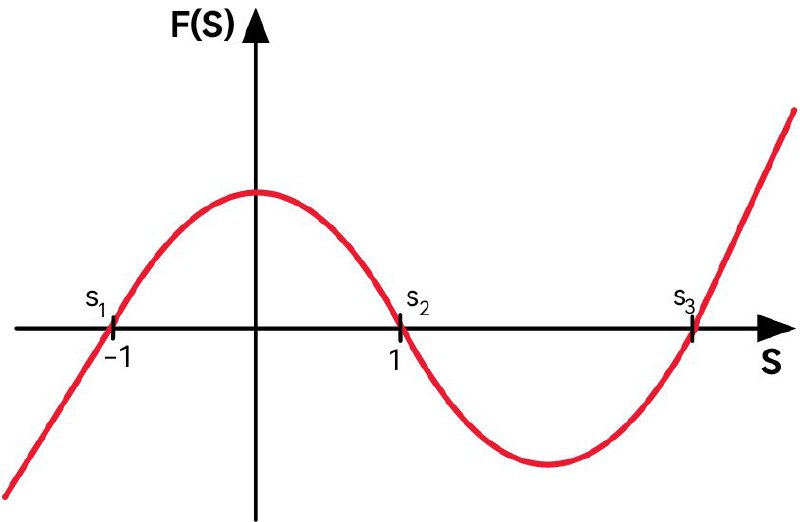
\includegraphics[width=0.8\linewidth]{images/лекция_10_2.jpeg}
\end{wrapfigure}
Рассмотрим $F(S)$ как функцию. Тогда
\[
S = \pm 1 \Longrightarrow F(S) \leq 0
\]
\[
S \in [-1,~ 1] \Longrightarrow F(S) \geq 0
\]
\[
S\longrightarrow\pm\infty \Longrightarrow F(S) \longrightarrow\pm\infty
\]
\begin{wrapfigure}{l}{0.3\textwidth}
  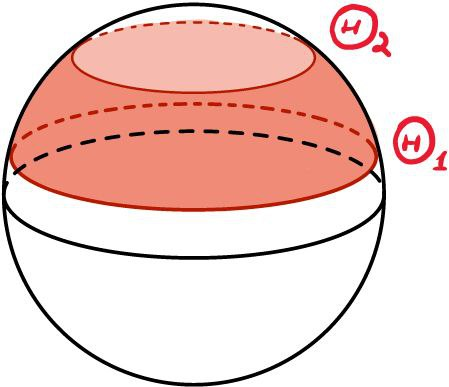
\includegraphics[width=0.8\linewidth]{images/лекция_10_3.jpeg}
\end{wrapfigure}

\tab\\ \tab\\ \tab\\

Итого, $\Theta_1$ и $\Theta_2$ --- углы, между которыми может находиться движение апекса. Т.е. волчок движется так, что косинус угла нутации $\Theta$ периодически меняется между этими значениями.\\

Вернемся к рассмотрению угловой скорости прецессии $\dot{\psi}$. Она является однозначной функцией угла нутации, а значит, изменяется с тем же периодом. Тогда возможны три случая, показанные на \hyperref[lecture_10_4]{рисунке}.

\begin{figure}[!h]
    \centering
    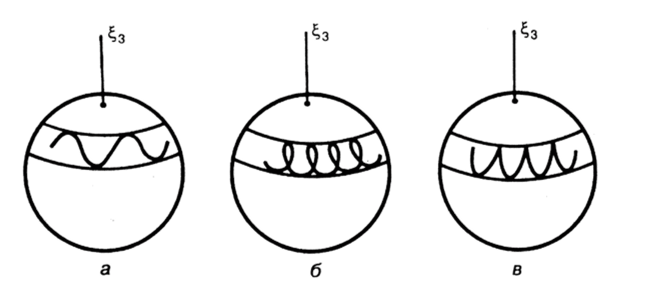
\includegraphics[width=0.75\linewidth]{images/лекция_10_4.png}
    \label{lecture_10_4}
\end{figure}

\begin{itemize}
    \item[a)] $\dot{\psi}(0) > 0$, в каждой точке траектории скорость прецессии положительна.
    \item[б)] $\dot{\psi}(0) < 0$, в нижних точках траектории скорость прецессии положительна, а в верхних --- отрицательна.
    \item[в)] $\dot{\psi}(0) = 0$, в нижних точках траектории скорость прецессии положительна и максимальна, а в верхних ось волчка останавливается --- это \textbf{точки возврата}.
\end{itemize}

\begin{frame}{Прим. редактора.} Кому интересно, вот \href{https://www.youtube.com/watch?v=EjC3t14PdNw}{здесь} и \href{https://www.youtube.com/watch?v=pwy1A_chRsg}{здесь} можно посмотреть видео с демонстрацией движения волчка Лагранжа.\\ \end{frame}

\underline{Регулярная прецессия}\\
Получим необходимое условие регулярной прецессии тела --- \textbf{основное уравнение гироскопии}.\\

Достаточным условием будет выполнение уравнения гироскопии и условия $\Theta = const$. Из результатов, полученных выше, понятно, что $\dot{\phi} = \dot{\psi} = const$. $\Theta$ не меняется, значит, $\dot{\Theta} = 0$. При этом должно выполняться
\[
\dfrac{d \vec{K}_A}{d t} = \vec{M} = \vec{\omega}_2 \times \vec{K}_A
\]
Тогда
\[
\vec{K}_A = A\begin{pmatrix}
    p\\
    q\\
    0\\
\end{pmatrix} + C\begin{pmatrix}
    0\\
    0\\
    r\\
\end{pmatrix}
\]
\[
\vec{\omega}_r = \vec{\omega}_1 + \vec{\omega}_2\cos{\Theta} = \vec{\omega}_1\left(1 + \dfrac{\vec{\omega}_2}{\vec{\omega}_1}\cos{\Theta}\right)
\]
\[
\vec{\omega}_{pq} = \vec{\omega} - \vec{\omega}_r = \vec{\omega}_1 + \vec{\omega}_2 - \vec{\omega}_r = \vec{\omega}_2 - \vec{\omega}_1\dfrac{{\omega}_2}{\omega_1}\cos{\Theta}
\]
Подставив в выражение для момента, получим
\[
\vec{M}_A = \vec{\omega}_2 \times \vec{K}_A = \vec{\omega}_2 \times \left( A\left(\vec{\omega}_2 - \vec{\omega}_1\dfrac{{\omega}_2}{\omega_1}\cos{\Theta}\right) + C\vec{\omega}_1\left(1 + \dfrac{\vec{\omega}_2}{\vec{\omega}_1}\cos{\Theta})\right)\right)
\]
Итого, \textbf{основное уравнение гироскопии}:
\[
\vec{M}_A = \vec{\omega}_2 \times \vec{\omega}_1\left(C + (C - A)\dfrac{{\omega}_2}{\omega_1}\cos{\Theta}\right)
\]


